\begin{frame}
	\frametitle{Material}
	
	Material para armar estas slides:
	\begin{itemize}
		\item Cyrill Stachniss SLAM \url{https://youtu.be/BuRCJ2fegcc}
   		\item Cyrill Stachniss Factor Graph \url{https://youtu.be/uuiaqGLFYa4}
		\item Cyrill Stachniss Graph-based SLAM using Pose Graphs \url{https://youtu.be/uHbRKvD8TWg}
		\item Cyrill Stachniss Graph-Based SLAM with Landmarks \url{https://youtu.be/mZBdPgBtrCM}
        %\item Cyrill Stachniss Least Squares \url{https://youtu.be/yVd-QDy0K6k}
		%\item Cyrill Stachniss Robust Least Squares for Graph-Based SLAM \url{https://youtu.be/z60RbiY18I8}
		%\item Cyrill Stachniss Hierarchical Pose Graphs for SLAM \url{https://youtu.be/uRSow8nMEw8}
		\item Wolfram Burgard, Giorgio Grisetti, and Cyrill Stachniss: Graph-based SLAM \url{https://youtu.be/Alu59K8zvYs}
		\item Frank Dellaert \url{https://youtu.be/tm4E1o11kGo}
        \item Apunte Frank Dellaert and Michael Kaess \url{https://www.cs.cmu.edu/~kaess/pub/Dellaert17fnt.pdf}
        \item \url{http://ais.informatik.uni-freiburg.de/teaching/ss13/robotics/slides/16-graph-slam.pdf}
	\end{itemize}
	
\end{frame}

\begin{frame}
	\frametitle{Temario para estas slides}
	
	\begin{itemize}
		\item Graph-SLAM / Factor Graph
		\item Loop-Closure
		\item Bundle Adjustment
	\end{itemize}
	
\end{frame}

\begin{frame}
	\frametitle{¿Qué es SLAM?}
	
	Para que un robot móvil pueda navegar de manera autónoma es necesario que conozca su ubicación y cuente con una representación del entorno donde se encuentra. Estos problemas se conocen como el problema Localización y el problema de Mapeo. En el caso más general, donde no se cuenta con un la localización del robot ni con un mapa a priori del entorno, dichas problemas se abordan de manera simultánea. Esto da origen al problema de SLAM (\emph{Simultaneous Localizacion and Mapping}).
	\begin{block}{}
		SLAM es el problema de resolver la localización y el mapeo al mismo tiempo.
	\end{block}
	
\end{frame}


\begin{frame}
    \frametitle{Ejemplo de SLAM}
    
    \begin{figure}
        \subfloat[Realidad]
        {
            \fbox{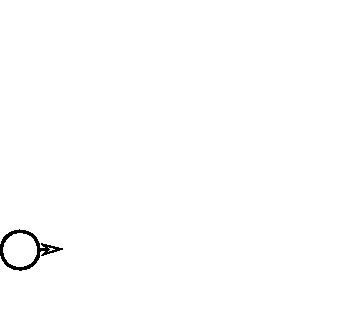
\includegraphics[width=0.44\textwidth]{slam_example_gt1.pdf}}
        }\hfill{}
        \subfloat[Sistema de SLAM del robot]
        {
            \fbox{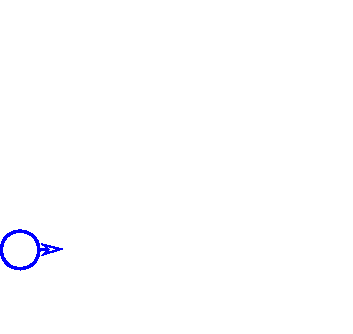
\includegraphics[width=0.44\textwidth]{slam_example_robot1.pdf}}
        }
    \end{figure}
    
\end{frame}

\begin{frame}
    \frametitle{Ejemplo de SLAM}
    
    \begin{figure}
        \subfloat[Realidad]
        {
            \fbox{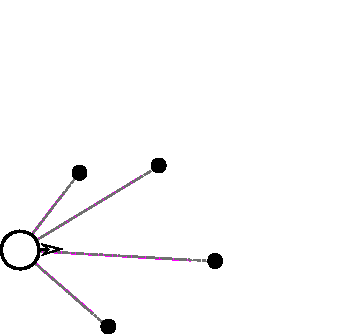
\includegraphics[width=0.44\textwidth]{slam_example_gt2.pdf}}
        }\hfill{}
        \subfloat[Sistema de SLAM del robot]
        {
            \fbox{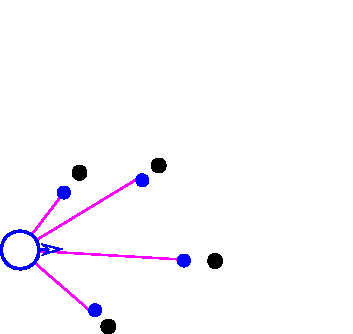
\includegraphics[width=0.44\textwidth]{slam_example_robot2.pdf}}
        }
    \end{figure}
    
\end{frame}

\begin{frame}
    \frametitle{Ejemplo de SLAM}
    
    \begin{figure}
        \subfloat[Realidad]
        {
            \fbox{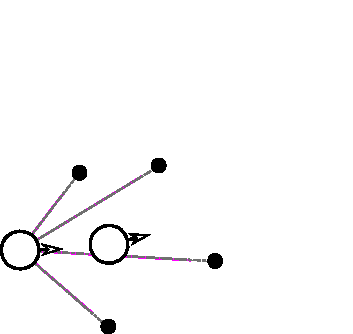
\includegraphics[width=0.44\textwidth]{slam_example_gt3.pdf}}
        }\hfill{}
        \subfloat[Sistema de SLAM del robot]
        {
            \fbox{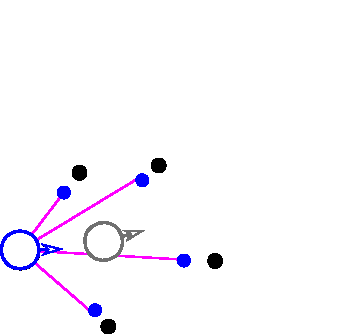
\includegraphics[width=0.44\textwidth]{slam_example_robot3.pdf}}
        }
    \end{figure}
    
\end{frame}

\begin{frame}
    \frametitle{Ejemplo de SLAM}
    
    \begin{figure}
        \subfloat[Realidad]
        {
            \fbox{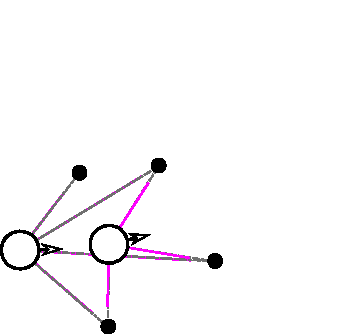
\includegraphics[width=0.44\textwidth]{slam_example_gt4.pdf}}
        }\hfill{}
        \subfloat[Sistema de SLAM del robot]
        {
            \fbox{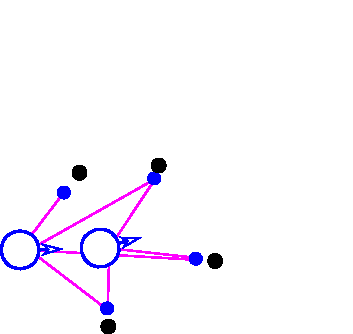
\includegraphics[width=0.44\textwidth]{slam_example_robot4.pdf}}
        }
    \end{figure}
    
\end{frame}

\begin{frame}
    \frametitle{Ejemplo de SLAM}
    
    \begin{figure}
        \subfloat[Realidad]
        {
            \fbox{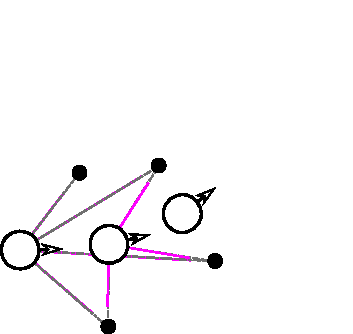
\includegraphics[width=0.44\textwidth]{slam_example_gt5.pdf}}
        }\hfill{}
        \subfloat[Sistema de SLAM del robot]
        {
            \fbox{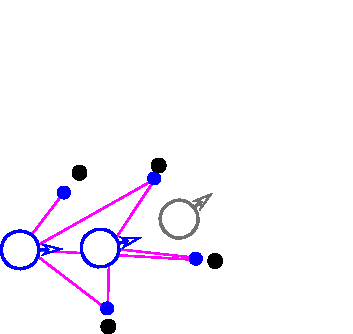
\includegraphics[width=0.44\textwidth]{slam_example_robot5.pdf}}
        }
    \end{figure}
    
\end{frame}

\begin{frame}
    \frametitle{Ejemplo de SLAM}
    
    \begin{figure}
        \subfloat[Realidad]
        {
            \fbox{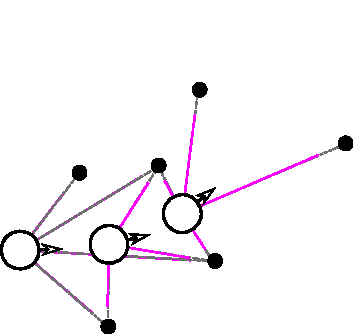
\includegraphics[width=0.44\textwidth]{slam_example_gt6.pdf}}
        }\hfill{}
        \subfloat[Sistema de SLAM del robot]
        {
            \fbox{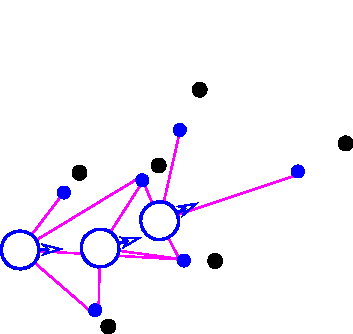
\includegraphics[width=0.44\textwidth]{slam_example_robot6.pdf}}
        }
    \end{figure}
    
\end{frame}

\begin{frame}
    \frametitle{Ejemplo de SLAM}
    
    \begin{figure}
        \subfloat[Realidad]
        {
            \fbox{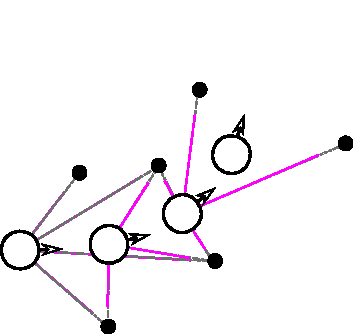
\includegraphics[width=0.44\textwidth]{slam_example_gt7.pdf}}
        }\hfill{}
        \subfloat[Sistema de SLAM del robot]
        {
            \fbox{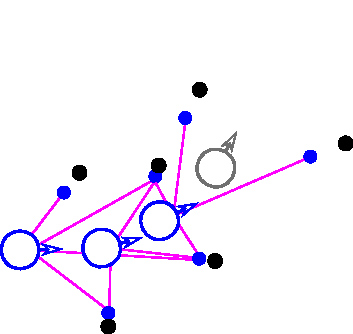
\includegraphics[width=0.44\textwidth]{slam_example_robot7.pdf}}
        }
    \end{figure}
    
\end{frame}

\begin{frame}
    \frametitle{Ejemplo de SLAM}
    
    \begin{figure}
        \subfloat[Realidad]
        {
            \fbox{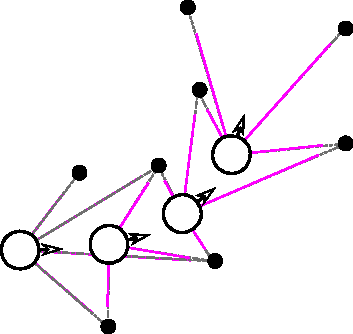
\includegraphics[width=0.44\textwidth]{slam_example_gt8.pdf}}
        }\hfill{}
        \subfloat[Sistema de SLAM del robot]
        {
            \fbox{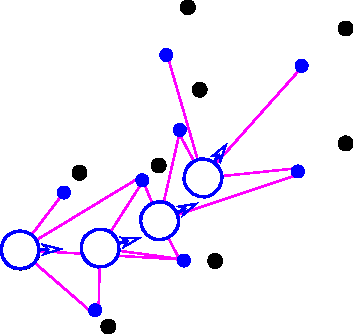
\includegraphics[width=0.44\textwidth]{slam_example_robot8.pdf}}
        }
    \end{figure}
    
\end{frame}

\begin{frame}
	\frametitle{Aquitectura general de SLAM}
	
	\begin{figure}[!h]
			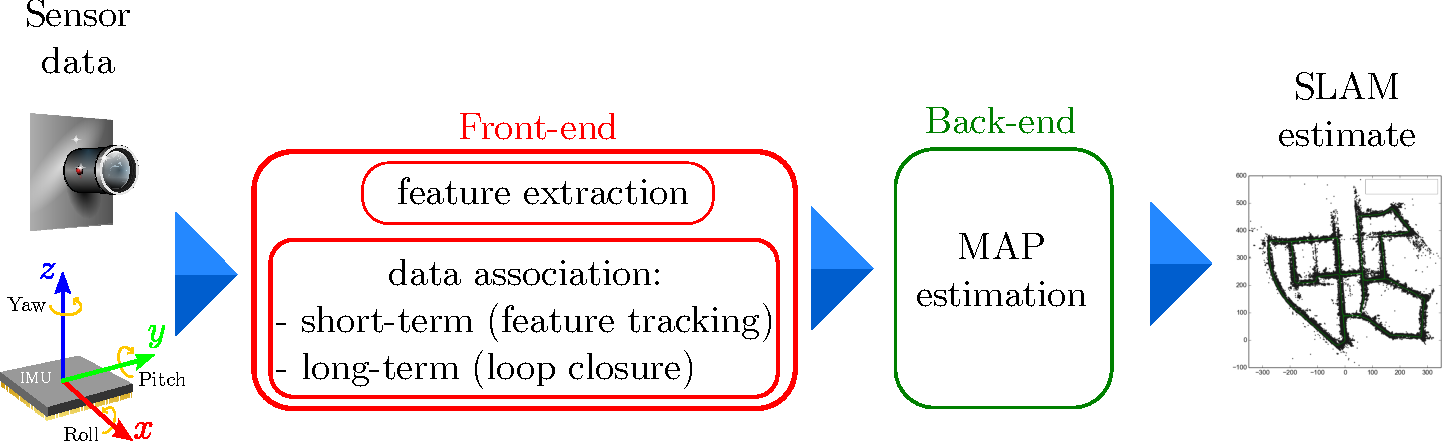
\includegraphics[width=\textwidth]{images/slam_frontend_backend.pdf}
	\end{figure}
	
\end{frame}

\begin{frame}
    \frametitle{Tipos de SLAM Back-ends}
    \note{Información extraída de https://youtu.be/BuRCJ2fegcc y de https://youtu.be/Alu59K8zvYs}
    \begin{itemize}
        \item Basados en Kalman Filter (EKF-SLAM)
        \item Basados en Particle Filter (FastSLAM, Rao-Blackwellized Particle Filter, Gmapping)
        \item Basados en Least-Squares (Graph-SLAM, Bundle Adjustment)
        \begin{itemize}
            \item Pose-Graph (solo contiene las poses del robot, el mapa es marginalizado)
            \item Factor-Graph (contiene poses y landmarks)
        \end{itemize}
            Herramientas de optimización
            \begin{itemize}
            \item Ceres
            \item GTSAM
            \item g2o
            \end{itemize}
    \end{itemize}

	\begin{figure}[!h]
        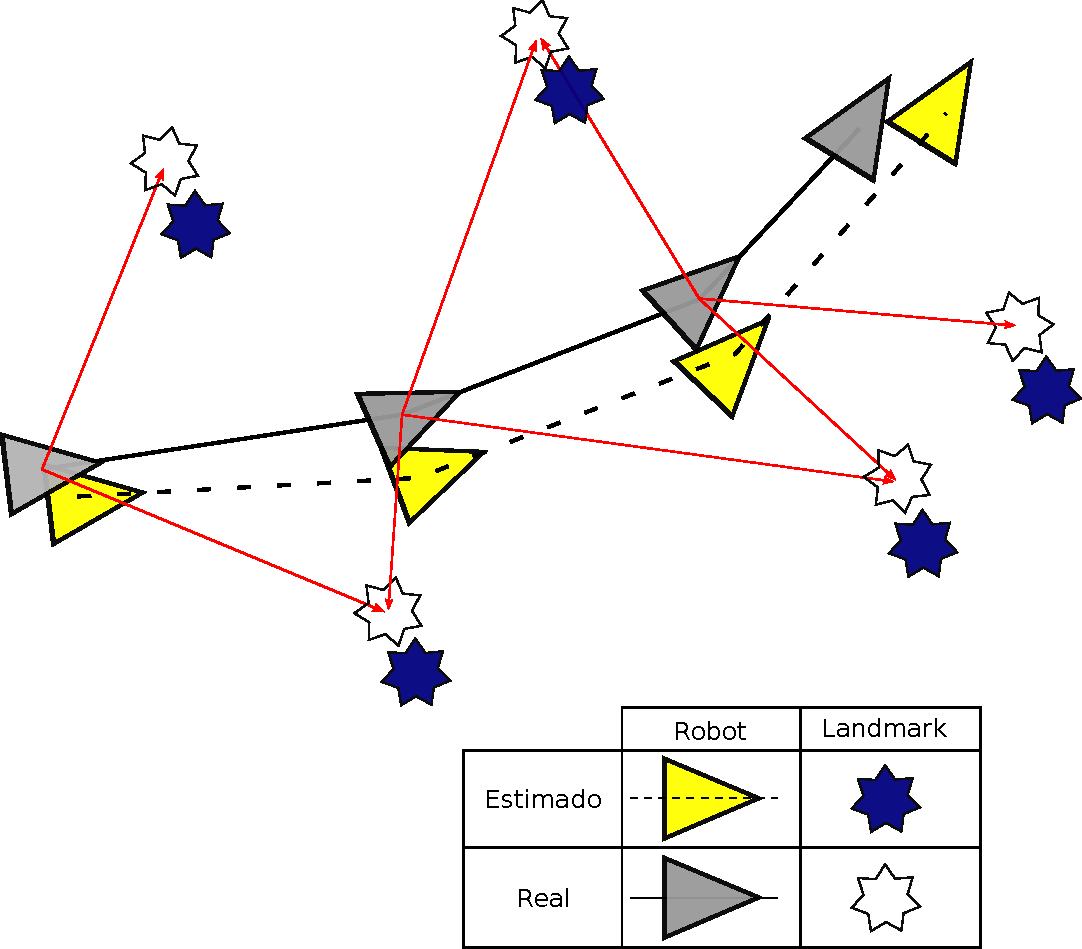
\includegraphics[width=0.2\textwidth]{images/slam-landmarks.pdf}
    \end{figure}
    
\end{frame}

\begin{frame}
    \frametitle{Graph-SLAM}
    
    Graph-SLAM: construir un grafo y encontrar una configuración de nodos que minimiza el error introducido por las restricciones (aristas)
    
    \begin{itemize}
        \item Se utiliza un grafo para representar el problema.
        \item Los nodos representan poses o ubicaciones de landmarks.
        \item Las aristas son observaciones de landmarks o mediciones de odometría
        \item La minimización optimiza las poses del robot y la ubicación del los landmarks
        \item Observar áreas previamente vistas genera restricciones en el grafo
    \end{itemize}

    \begin{figure}
    \subfloat[]
    {
        \fbox{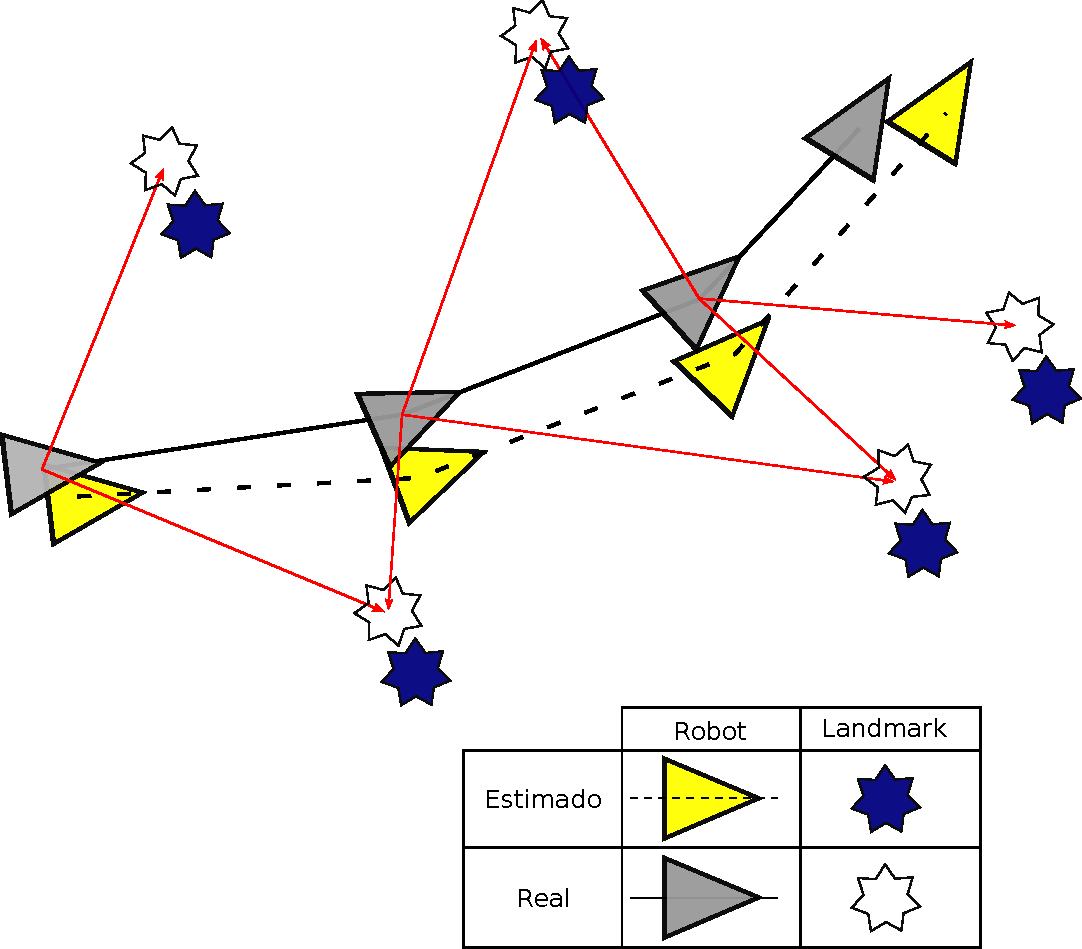
\includegraphics[width=0.25\textwidth]{images/slam-landmarks.pdf}}
    }\hspace{1em}
    \subfloat[]
    {
        \fbox{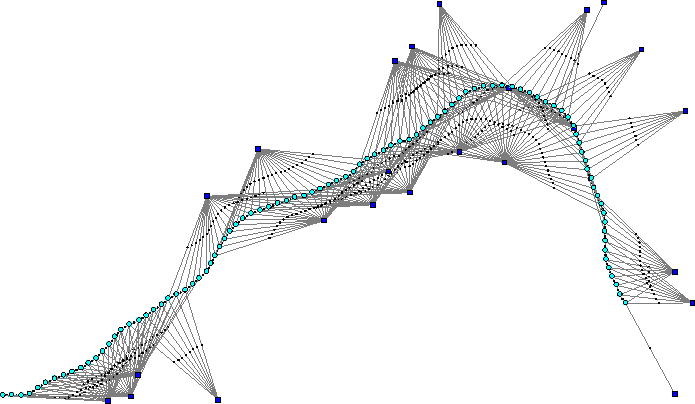
\includegraphics[width=0.375\textwidth]{images/factor_graph.pdf}}
    }
    \end{figure}
    
\end{frame}


\begin{frame}
    \frametitle{Factor-Graph}
    \note{Información extraída de https://youtu.be/uuiaqGLFYa4}
    
    \begin{block}{Factor-Graph}
        Un Factor-graph es un término matemático, un grafo bipartito representando la factorización de una función. Esto significa que podemos tomar una función por ejemplo $g(.)$ y descomponerla mediante el producto de funciones $f(.)$,
        
        \begin{equation*}
            g(X_{1}, \dots, X_{n}) = \prod_{i} f_{i}(S_{i}) \quad \text{con} \quad S_{i} 	\subseteq \{ X_{1},\dots, X_{n} \}
        \end{equation*}
    \end{block}

    \begin{figure}[!h]
        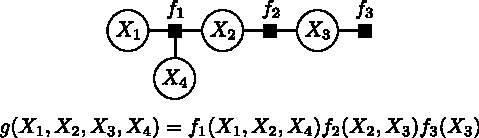
\includegraphics[width=0.7\textwidth]{images/factor_graph_example.pdf}
    \end{figure}

    \note{Por ejemplo, si la función g depende de 10 variables podemos descomponerla en el profucto de varias funciones f, donde cada función f depende de un subconjunto de esas variables.}
    
\end{frame}


\begin{frame}
    \frametitle{Factor-Graph}
    \note{Información extraída de https://youtu.be/uuiaqGLFYa4}
    
    \begin{itemize}
        \item Los Factor-Graph nos permiten representar una distribución de probabilidad conjunta (distribución que gobierna sobre todas las variables) como un producto de probabilidades más chicas (que dependen de un menor número de variables).
        \item Al igual que las redes de Bayes o redes de Markov, podemos utilizar los Factor-Graph para describir cómo las variables dependen entre si. Y podemos correr diferentes algoritmos sobre estos Factor-Graph para inferir información de una manera eficiente.
        \item Ejemplo de algorimo que trabaja sobre Factor-graph, es el Algoritmo de Sum-product para el computo de distribuciones marginales (distribuciones que solamente dependen un subconjunto de variables).
        \item En el contexto de robótica los Factor-graph son utilizados para especificar problemas de mínimos cuadrados. El factor graph nos permite representar cómo ciertos estados dependen o estan relacionados entre sí basados en la información que tenemos de las mediciones de los sensores (almacenada en los factores).
    \end{itemize}
    
    \note{Por ejemplo, si la función g depende de 10 variables podemos descomponerla en el profucto de varias funciones f, donde cada función f depende de un subconjunto de esas variables.}
    
\end{frame}

\begin{frame}
    \frametitle{Graph-based SLAM usando Pose-Graph}
    \note{Información extraída de https://youtu.be/uHbRKvD8TWg}
    \begin{itemize}
		\item asdf
    \end{itemize}
    
\end{frame}

\begin{frame}
    \frametitle{Graph-based SLAM usando Pose-Graph}
    \note{Información extraída de https://youtu.be/uHbRKvD8TWg}
    
\end{frame}

\begin{frame}
    \frametitle{Graph-based SLAM usando Pose-Graph}
    \note{Información extraída de https://youtu.be/uHbRKvD8TWg}
    
    \begin{columns}
        \begin{column}{0.5\textwidth}
        \begin{itemize}
            \item<1-2> Cada nodo es una pose del robot junto con su medición de laser (no hay landmarks)
            \item<1-2> Cada arista corresponde a una restricción espacial entre los nodos que relaciona.
            \item<3-> Una vez que tenemos el grafo, obtenemos el mapa mas probable mediante la corrección de los nodos
            \item<4-> así...
            \item<5> Dibujamos el mapa basandonos en las poses corregidas
        \end{itemize}
        \end{column}
        \begin{column}{0.5\textwidth}  %%<--- here
                \only<1>{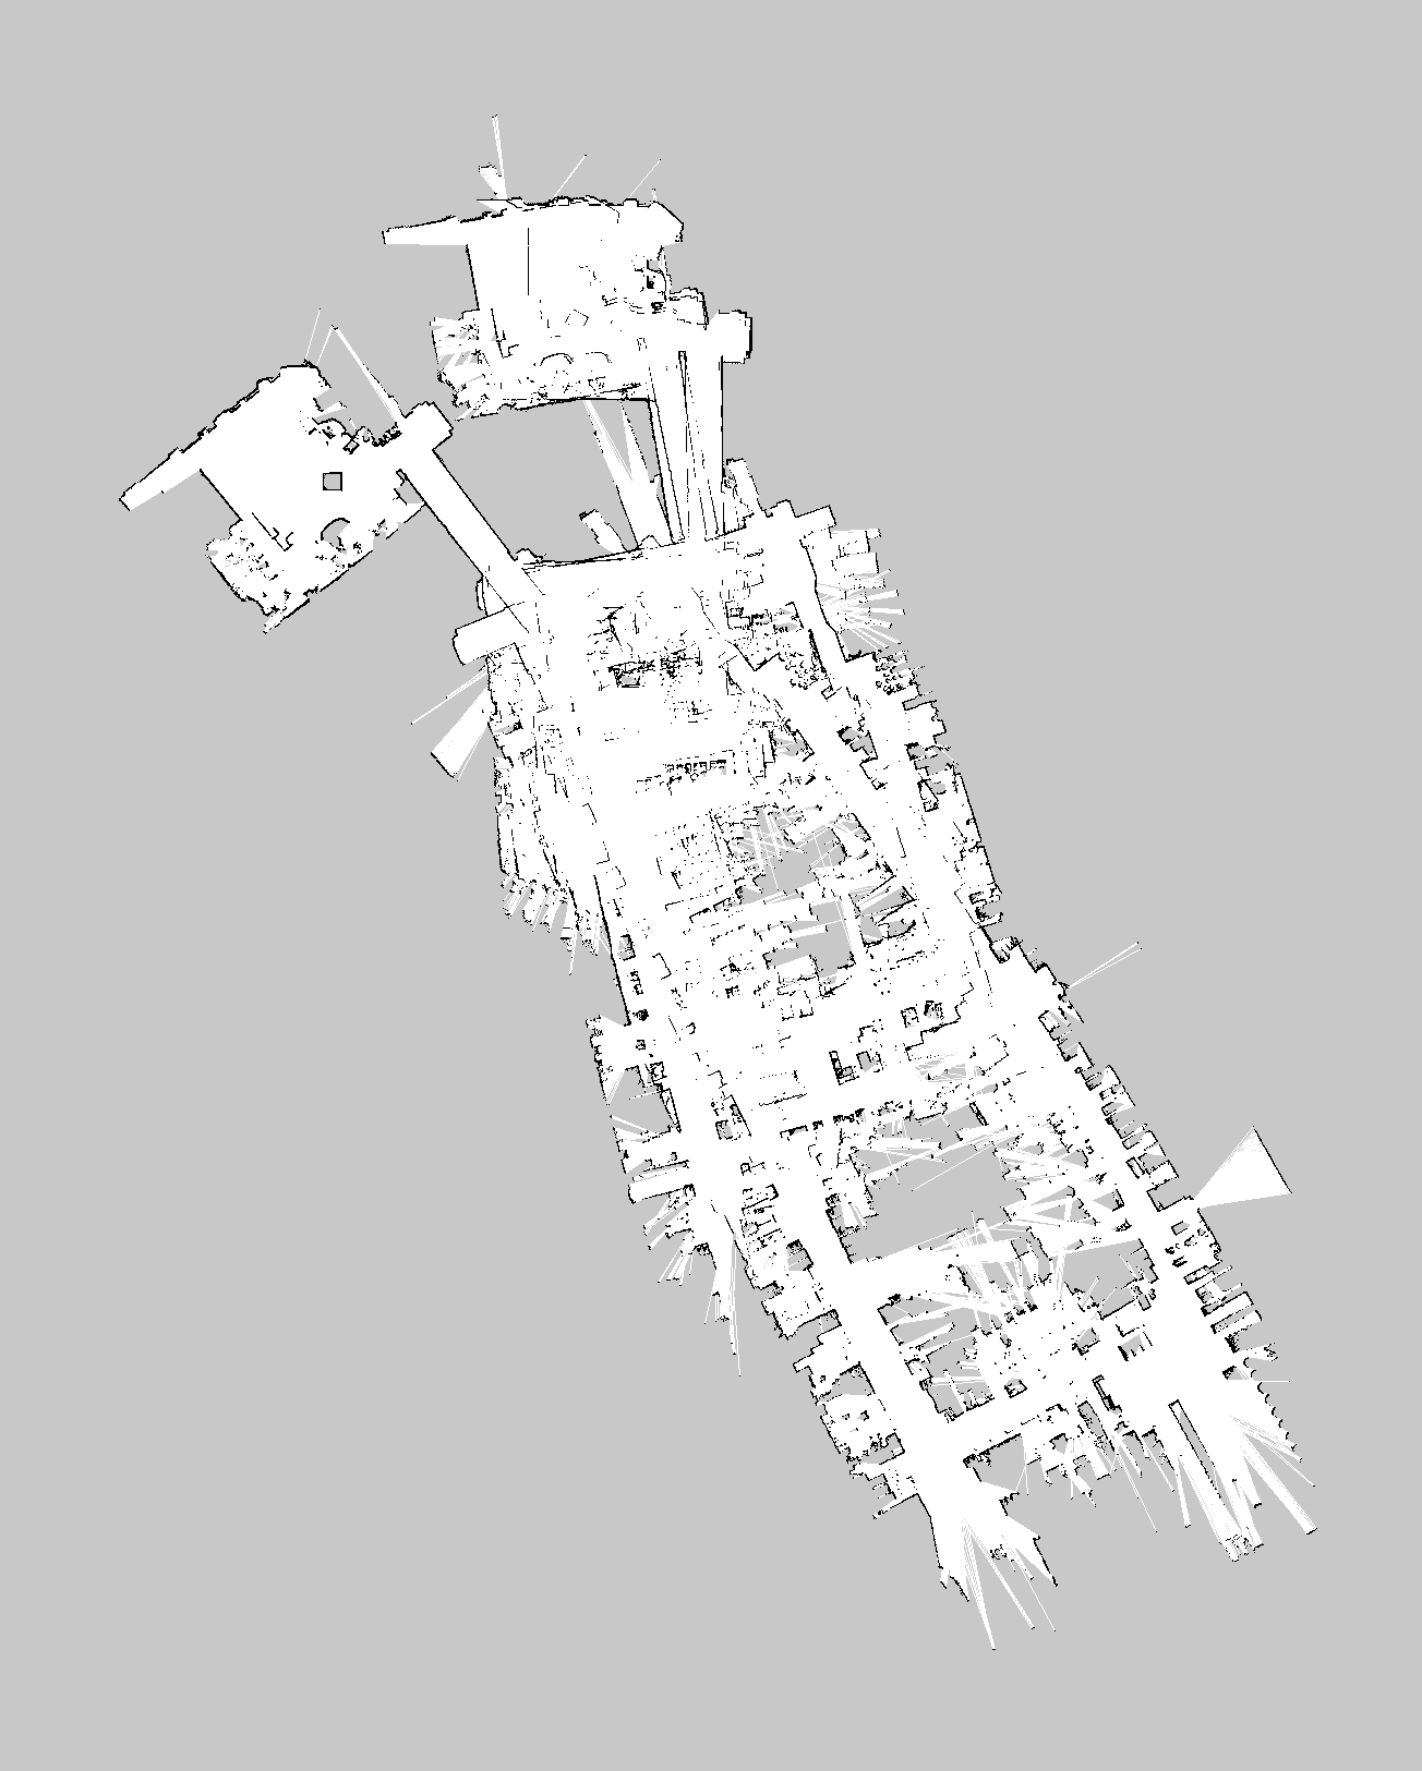
\includegraphics[width=0.7\textwidth]{images/pose_graph_map.png}}
                \only<2>{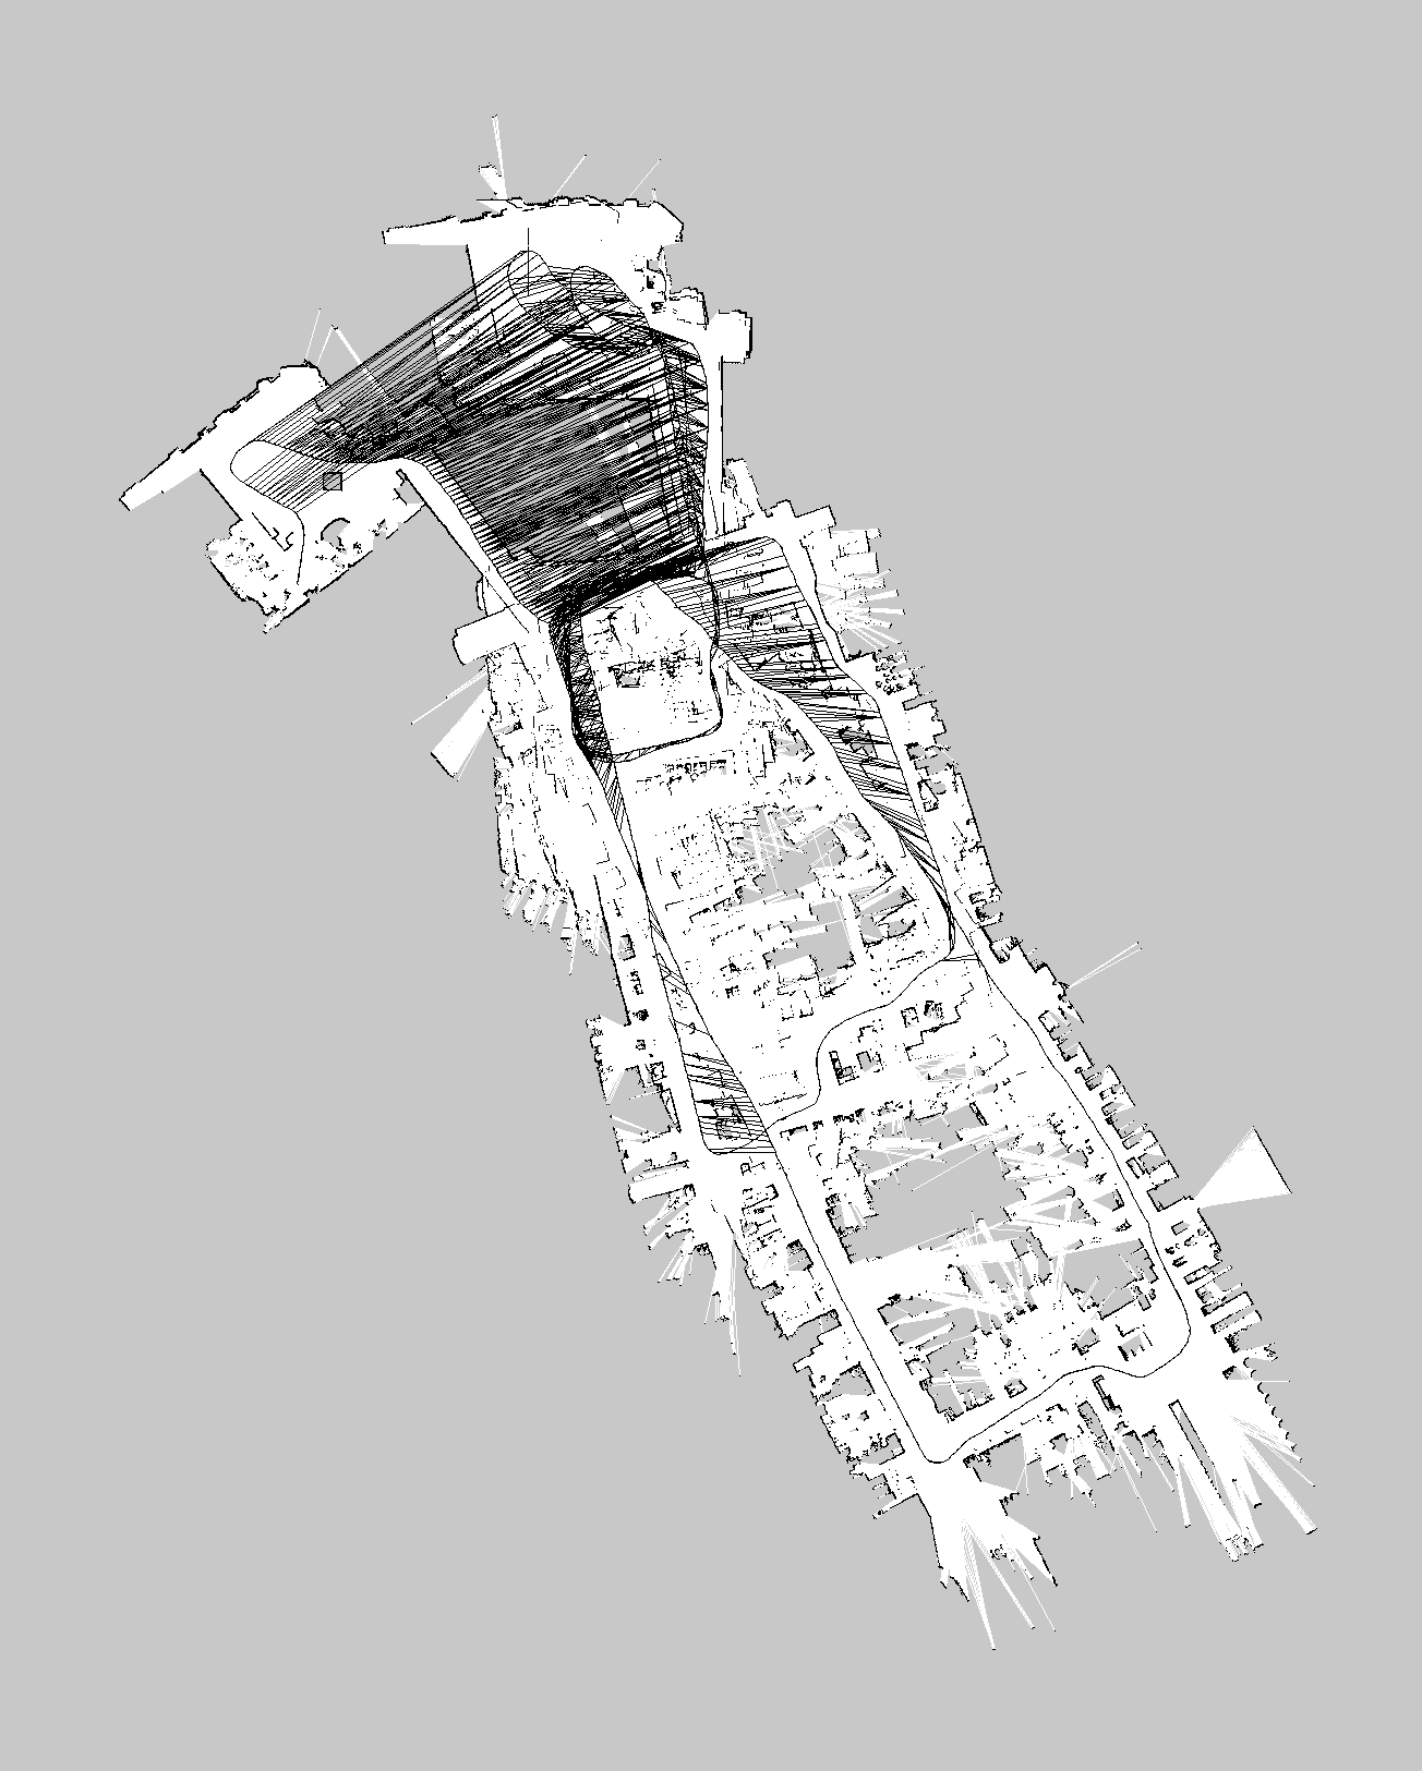
\includegraphics[width=0.7\textwidth]{images/pose_graph_constraints_with_map.png}}
                \only<3>{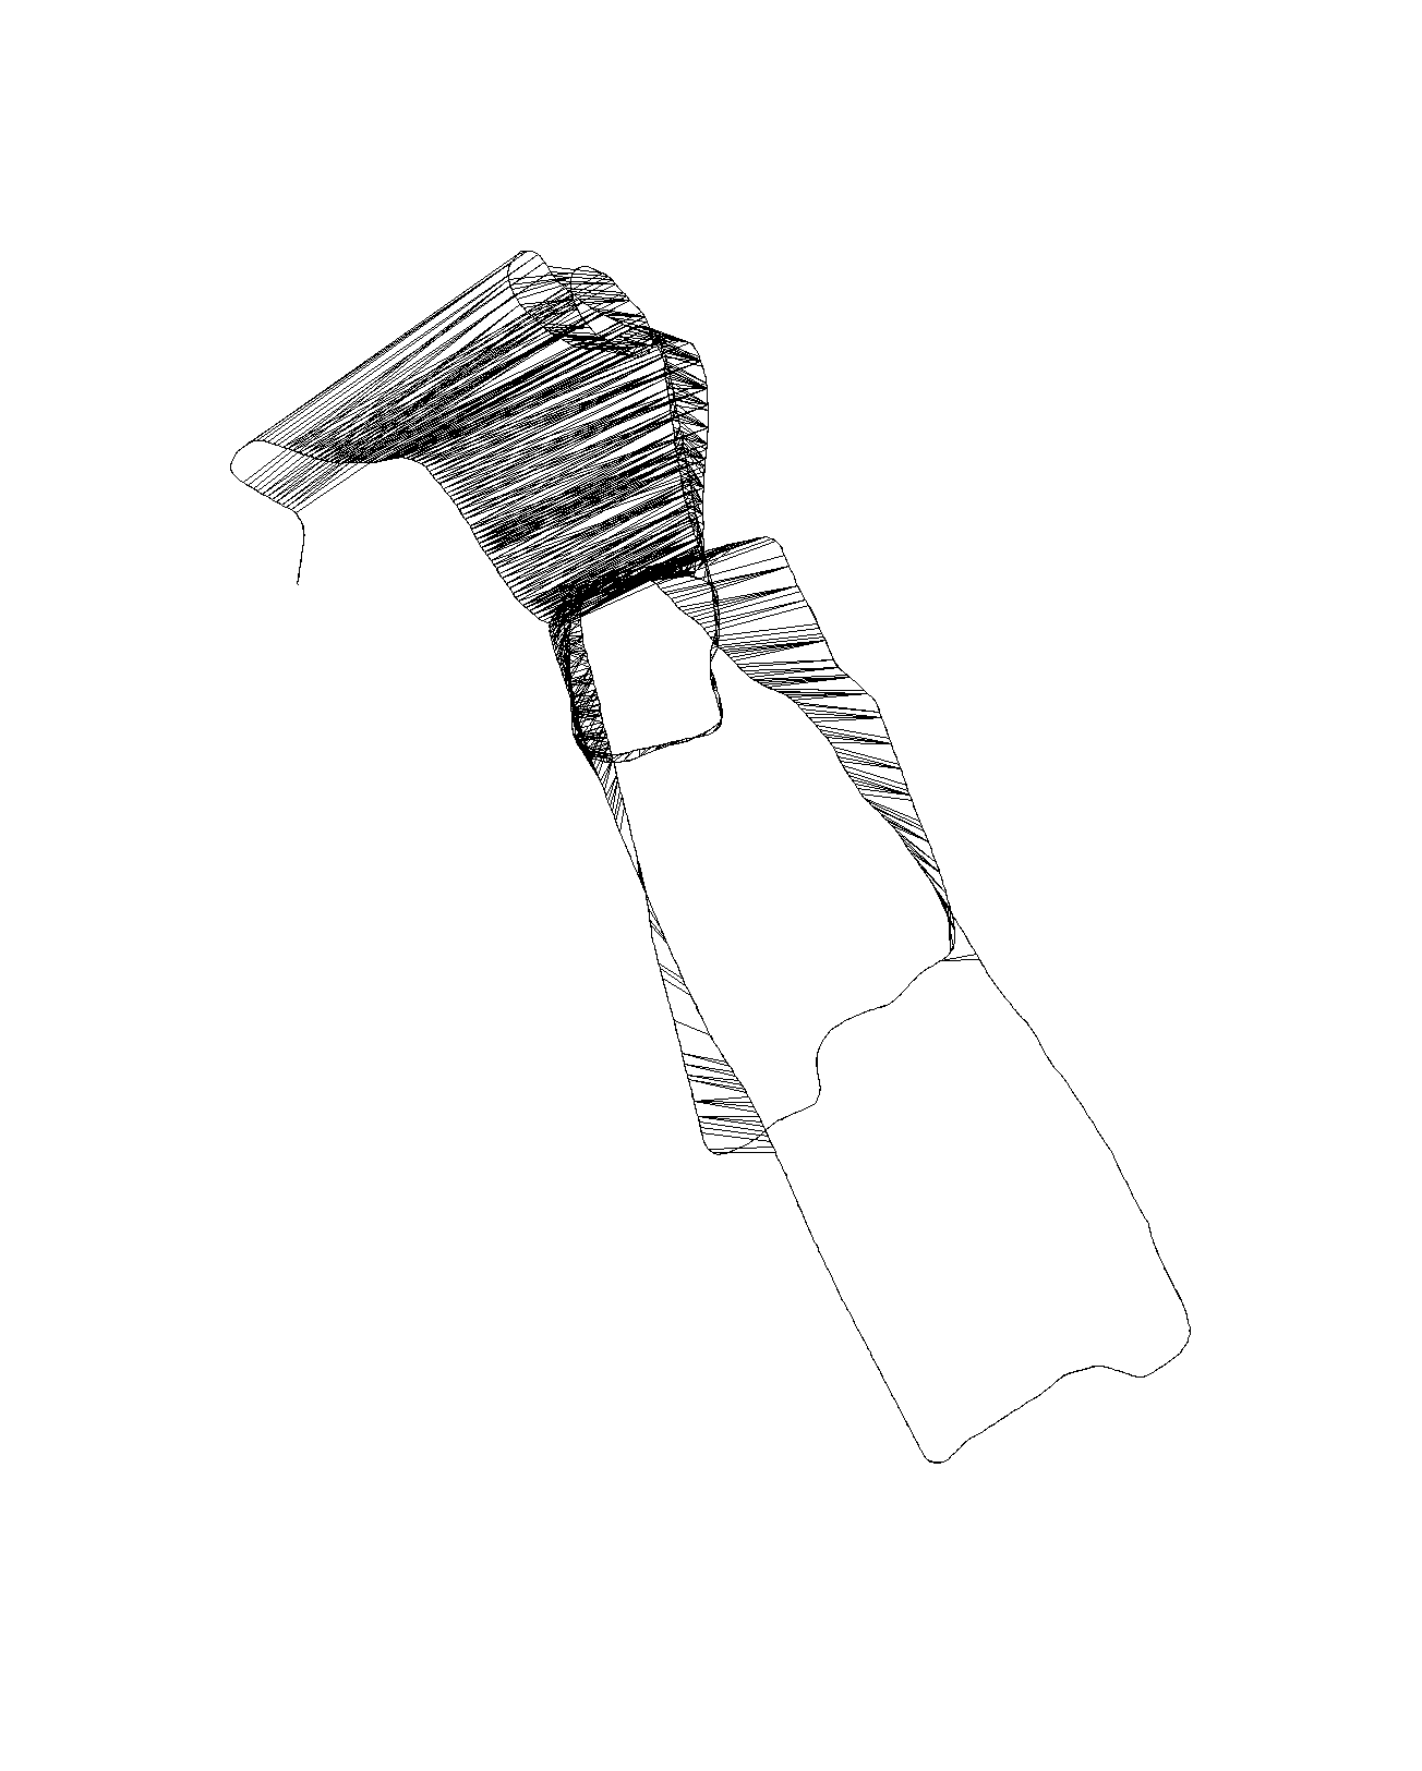
\includegraphics[width=0.7\textwidth]{images/pose_graph_constraints.png}}
                \only<4>{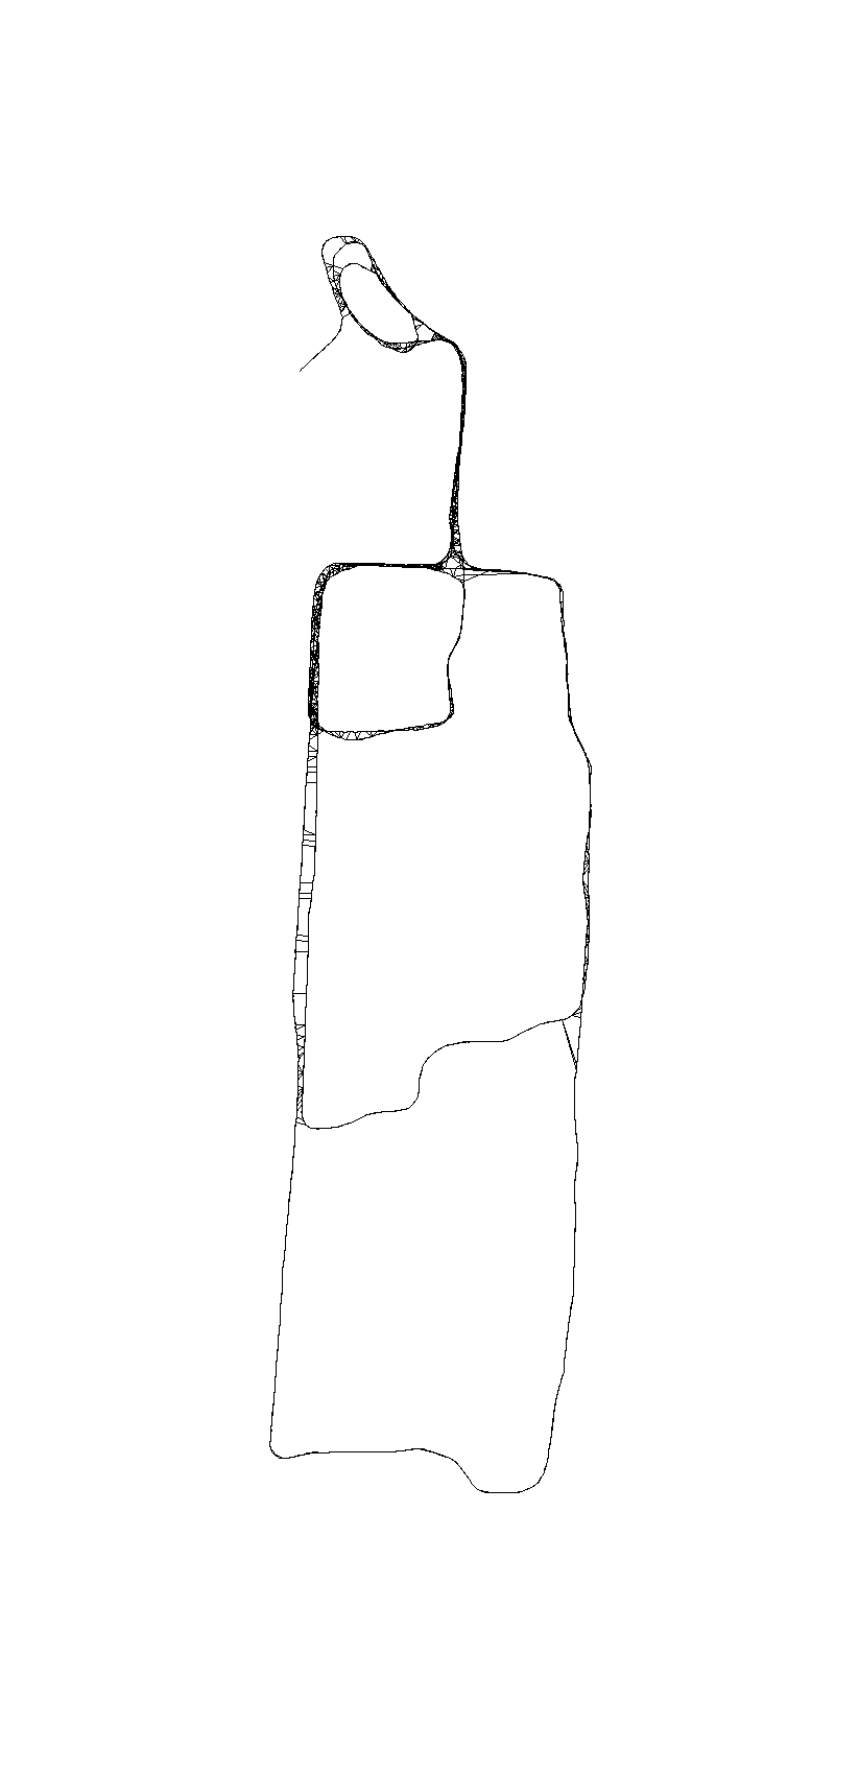
\includegraphics[width=0.5\textwidth]{images/pose_graph_optimized.png}}
                \only<5>{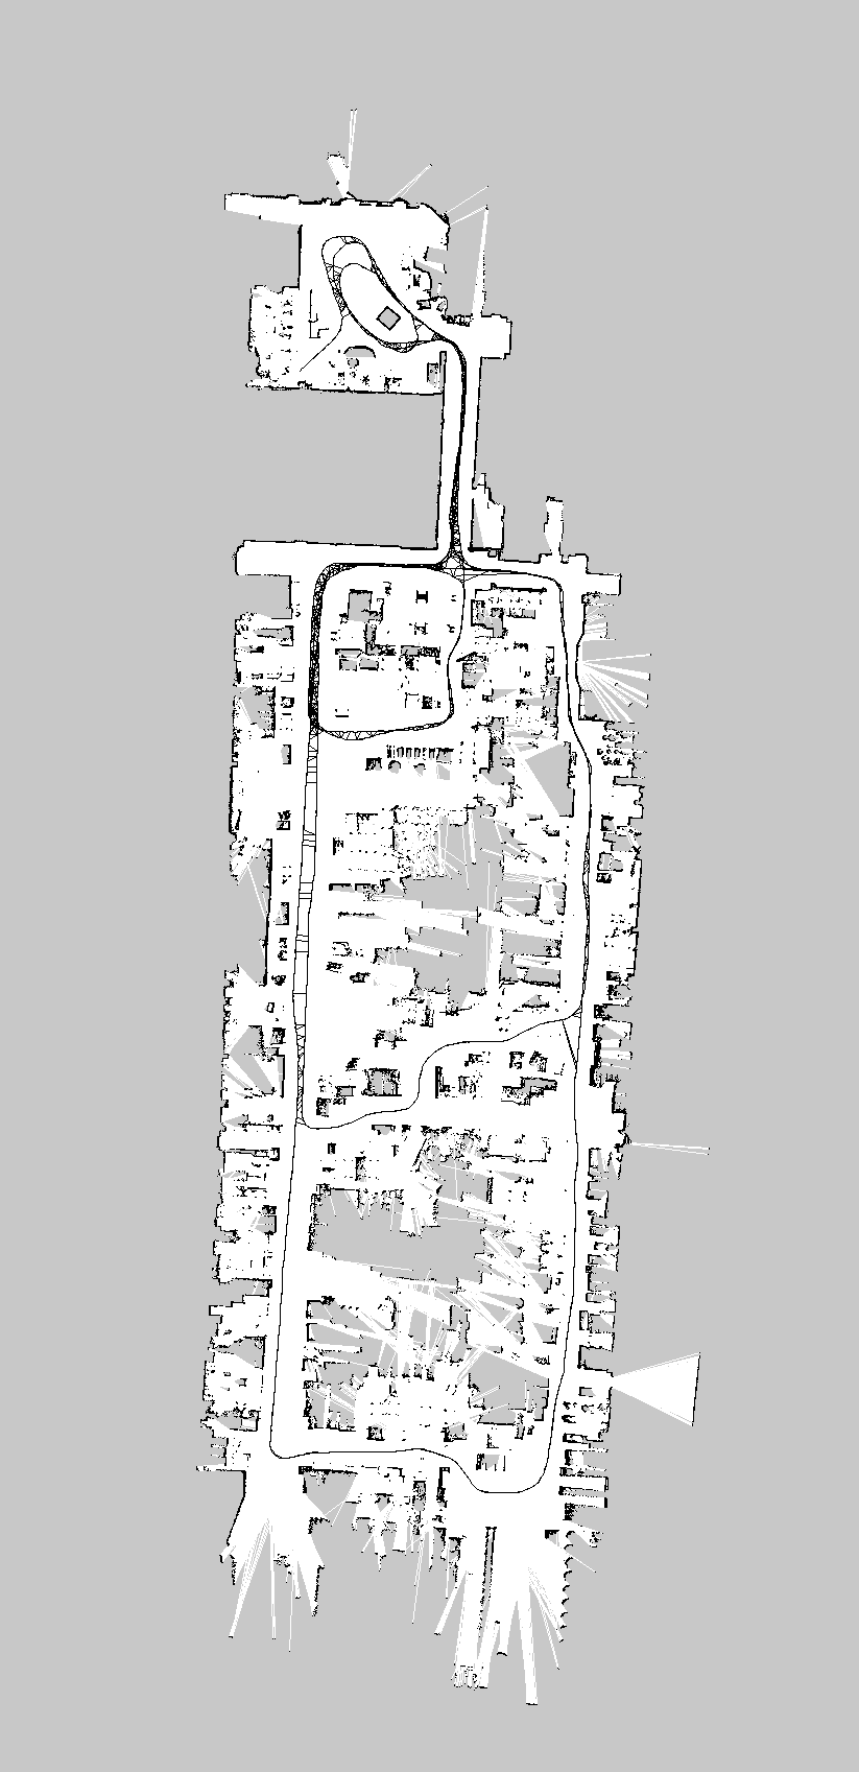
\includegraphics[width=0.5\textwidth]{images/pose_graph_optimized_with_map.png}}
        \end{column}
    \end{columns}
    
\end{frame}

\begin{frame}
	\frametitle{Graph-based SLAM usando Pose-Graph}
	\note{Información extraída de https://youtu.be/uHbRKvD8TWg}
	\begin{itemize}
		\item asdf
	\end{itemize}
	
	\begin{figure}[!h]
		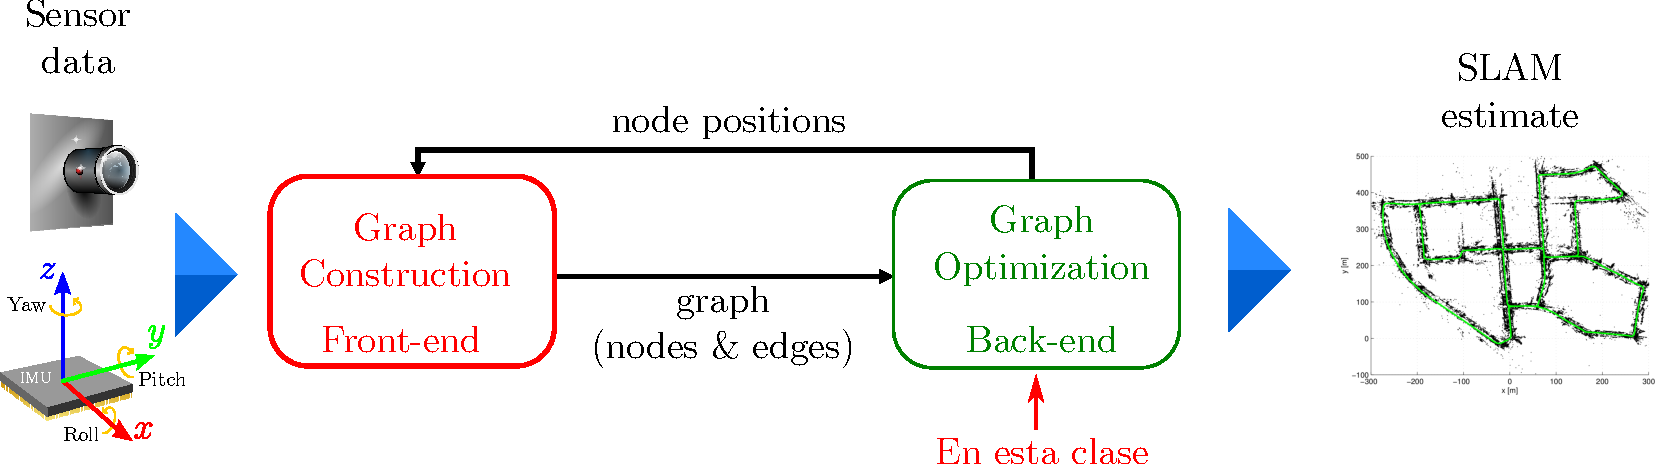
\includegraphics[width=\textwidth]{images/slam_frontend_backend_graph.pdf}
	\end{figure}
	
\end{frame}

\begin{frame}
    \frametitle{Graph-based SLAM usando Pose-Graph}
    \note{Información extraída de https://youtu.be/uHbRKvD8TWg}
    
    \begin{columns}
        \begin{column}{0.5\textwidth}
            \begin{itemize}
                \item Cada nodo es una pose del robot (no hay landmarks)
                \item Cada arista corresponde a una restricción espacial entre los nodos que relaciona.
            \end{itemize}
        \end{column}
        \begin{column}{0.5\textwidth}  %%<--- here
            \begin{figure}[!h]
                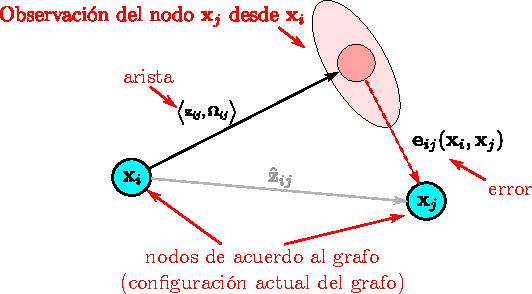
\includegraphics[width=0.7\textwidth]{images/factor_graph_edge_example.pdf}
            \end{figure}
        \end{column}
    \end{columns}
    
\end{frame}


\begin{frame}
    \frametitle{Graph-Based SLAM con landmarks}
    \note{Información extraída de https://youtu.be/mZBdPgBtrCM}
    
\end{frame}


\begin{frame}
    \frametitle{Bundle Adjustment}
    \note{Información extraída de https://youtu.be/BuRCJ2fegcc y de https://youtu.be/mZBdPgBtrCM}
    
    Bundle Adjustment es un caso
    
    \begin{itemize}
        \item Reconstrucción 3D basada en imágenes tomadas de diferentes puntos de vista
        \item Minimiza el error de reproyección en el plano de la imagen 2D
        \item No hay noción de odometría (pose-pose constraints)
        \item En general utiliza como método de minimización Levenberg-Marquart
        \item Desarrollado en el área de Fotogrametría\footnote{Fotogrametría es la técnica cuyo objeto es estudiar y definir con precisión la forma, dimensiones y posición en el espacio de un objeto cualquiera, utilizando esencialmente medidas hechas sobre una o varias fotografías de ese objeto} durante la década de 1950
    \end{itemize}
    
\end{frame}


